\appendix
\renewcommand{\thechapter}{C}
\chapter{Speckle beam width in the focal plane from a ray optics model}
\label{appendix:beam_width}

The speckle beam width in the focal plane of a lens can be calculated from a ray optics model, in the limit of large focal length $f$ and small diverging angle $\Delta \theta$.

\begin{figure}[htbp]
    \centering
    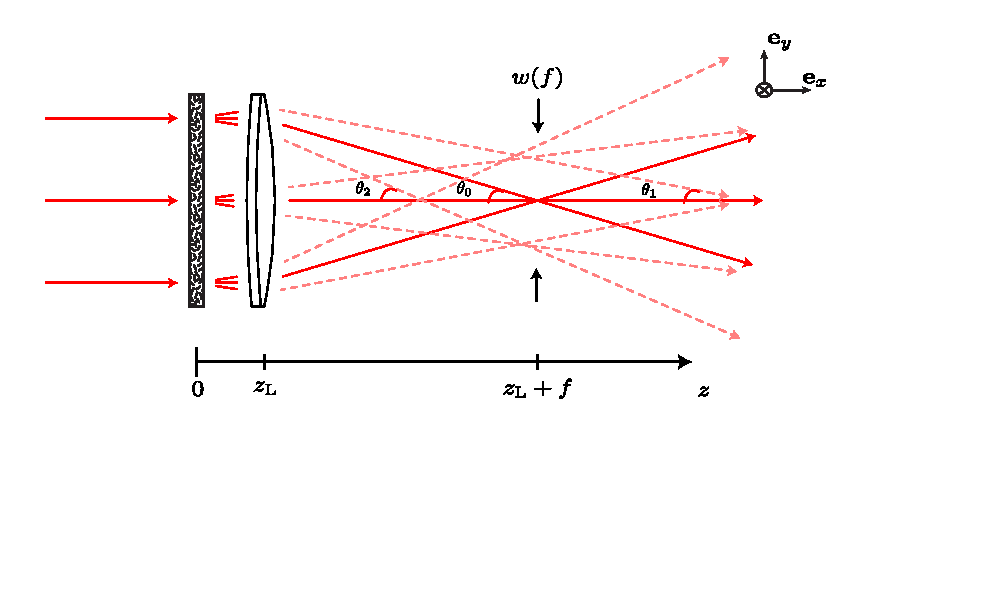
\includegraphics[width=\textwidth]{Fig1_appen.pdf}
    \caption{A ray optics model to calculate the speckle beam width in the focal plane of a lens.}
    \label{fig:append1}
\end{figure}

As shown in Fig.~\ref{fig:append1}, an optical ray hit the edge of a lens is focused to the focal point and form an angle $theta_0$ with $x$-axis. After the phase plate the speckle beam diverges at an angle $\Delta \theta$, and the diverged beam form angles $\theta_1$ and $theta_2$ with the $x$-axis.

\begin{align}
    \theta_1 &\approx \theta_0 - \Delta \theta\\\nonumber
    \theta_2 &\approx \theta_0 + \Delta \theta\\\nonumber
    f &= \frac{D_L}{2\tan{\theta_0}}\\\nonumber
\end{align}

For small $\Delta \theta$,
\begin{align}
    w(f) &= D_L \frac{\tan{\theta_2}-\tan{\theta_1}}{\tan{\theta_2}+\tan{\theta_1}}\\\nonumber
    & \approx D_L \frac{\sec{\theta_0}^2 \Delta \theta}{\tan{\theta_0}}\\\nonumber
    & = \frac{D_L\Delta \theta}{\sin{\theta_0}\cos{\theta_0}}\\\nonumber
\end{align}

In the limit of large $f$, $\sin{\theta_0} \approx \frac{D_L}{2f}$, $\cos{\theta_0} \approx 1$.
\begin{equation}
    w(f) \approx 2f\Delta \theta.
\end{equation}
